\section{Materials and Methods}
\subsection{Link Budget Analysis} \label{sec:link_budget}
Downlink communications from LEO face challenges associated with link geometry and the propagation environment. While orbital altitudes are substantially lower than geostationary systems, free-space path losses remain significant and vary with the elevation angle. Additional impairments include electromagnetic interference from co-existing systems and atmospheric and ionospheric effects that cause signal attenuation and fluctuations. These conditions, combined with the limited transmit power available on CubeSat platforms, impose tight design margins.

A link budget analysis was carried out to determine the minimum elevation angle at which reliable communication is feasible for a fixed channel bandwidth of 2\,MHz, evaluating three modulation schemes: QPSK, 8PSK, and 16PSK. These schemes were selected for their constant or near-constant envelope, which limits amplitude variations in the transmitted signal and reduces the risk of driving the amplifier into its nonlinear region \cite{Cripps2006}. For a roll-off factor of $\alpha = 0.35$, this bandwidth yields symbol rates and achievable data rates of 2.96\,Mbps for QPSK, 4.44\,Mbps for 8PSK, and 5.93\,Mbps for 16PSK. The calculations were performed following the methodology described in \cite{Seybold2005}, implemented in a Python script that allowed parametric tuning of the system parameters. The assumed values are listed in Table~\ref{tab:link_budget_params}.

\begin{table}[b]
    \caption{Link Budget Parameters}
    \label{tab:link_budget_params}
    \centering
    \renewcommand{\arraystretch}{1.15}
    \begin{tabular}{lcc}
        \hline\hline
        \textbf{Parameter} & \textbf{Symbol} & \textbf{Value} \\
        \hline
        Bandwidth               & $BW$               & 2\,MHz   \\
        Transmit power          & $P_T$              & 0\,dBW   \\
        TX antenna gain         & $G_T$              & 7\,dBi   \\
        RX antenna gain         & $G_R$              & 27\,dBi  \\
        Transmitter losses      & $L_{TX}$           & 1\,dB    \\
        Pointing loss           & $L_\text{point}$   & 1\,dB    \\
        Atmospheric losses      & $L_\text{atm}$     & 1\,dB    \\
        Antenna noise temp.     & $T_\text{ant}$     & 55\,K    \\
        LNA noise temp.         & $T_\text{LNA}$     & 70\,K    \\
        Orbital altitude        & $h$                & 600\,km  \\
        \hline\hline
    \end{tabular}
\end{table}

Free-space path loss was computed from the satellite-to-ground distance $D(\epsilon)$, given by \eqref{eq_D}

\begin{equation}
    D = \sqrt{(r_E + h)^2 - r_E^2 \cos^2{\epsilon}} - r_E \sin{\epsilon}
    \label{eq_D}
\end{equation}

where $r_E$ is Earth's mean radius, $h = 600\,\text{km}$ is the orbital altitude, corresponding to the region of highest orbital object density in LEO (600--800\,km)~\cite[Sec.~1.3.1]{AnzMeador2018}, and $\epsilon$ is the elevation angle. For each modulation scheme, a 1\,dB margin above the minimum $E_b/N_0$ required for a bit error rate (BER) of $10^{-5}$ was imposed.

The operating frequency was set to 2.2\,GHz, in proximity to both the 2170--2200\,MHz band allocated to the Mobile Satellite Service (MSS) for downlinks and the 2200--2290\,MHz band designated for space research, as defined by the ITU Radio Regulations~\cite{ITU_RR2024}. Operating near this boundary ensures spectral compatibility with MSS systems while remaining aligned with frequencies used in space exploration and research missions.

Fig.~\ref{fig:link_budget} shows the available $E_b/N_0$ as a function of elevation angle for each modulation scheme, alongside the corresponding minimum required $E_b/N_0$ indicated by horizontal dashed lines. QPSK becomes viable above an elevation angle of 20$\degree$, requiring a minimum $E_b/N_0$ of 10.6\,dB. 8PSK requires 14.3\,dB, achievable above 51$\degree$. 16PSK demands 19.3\,dB, a threshold that is not reached within the elevation range considered under the assumed link parameters, making it unsuitable for this configuration. These results support the adoption of adaptive modulation schemes, switching between QPSK and 8PSK as a function of satellite elevation, to maximize throughput while maintaining a reliable link margin throughout the pass.

\begin{figure}[t]
    \centering
    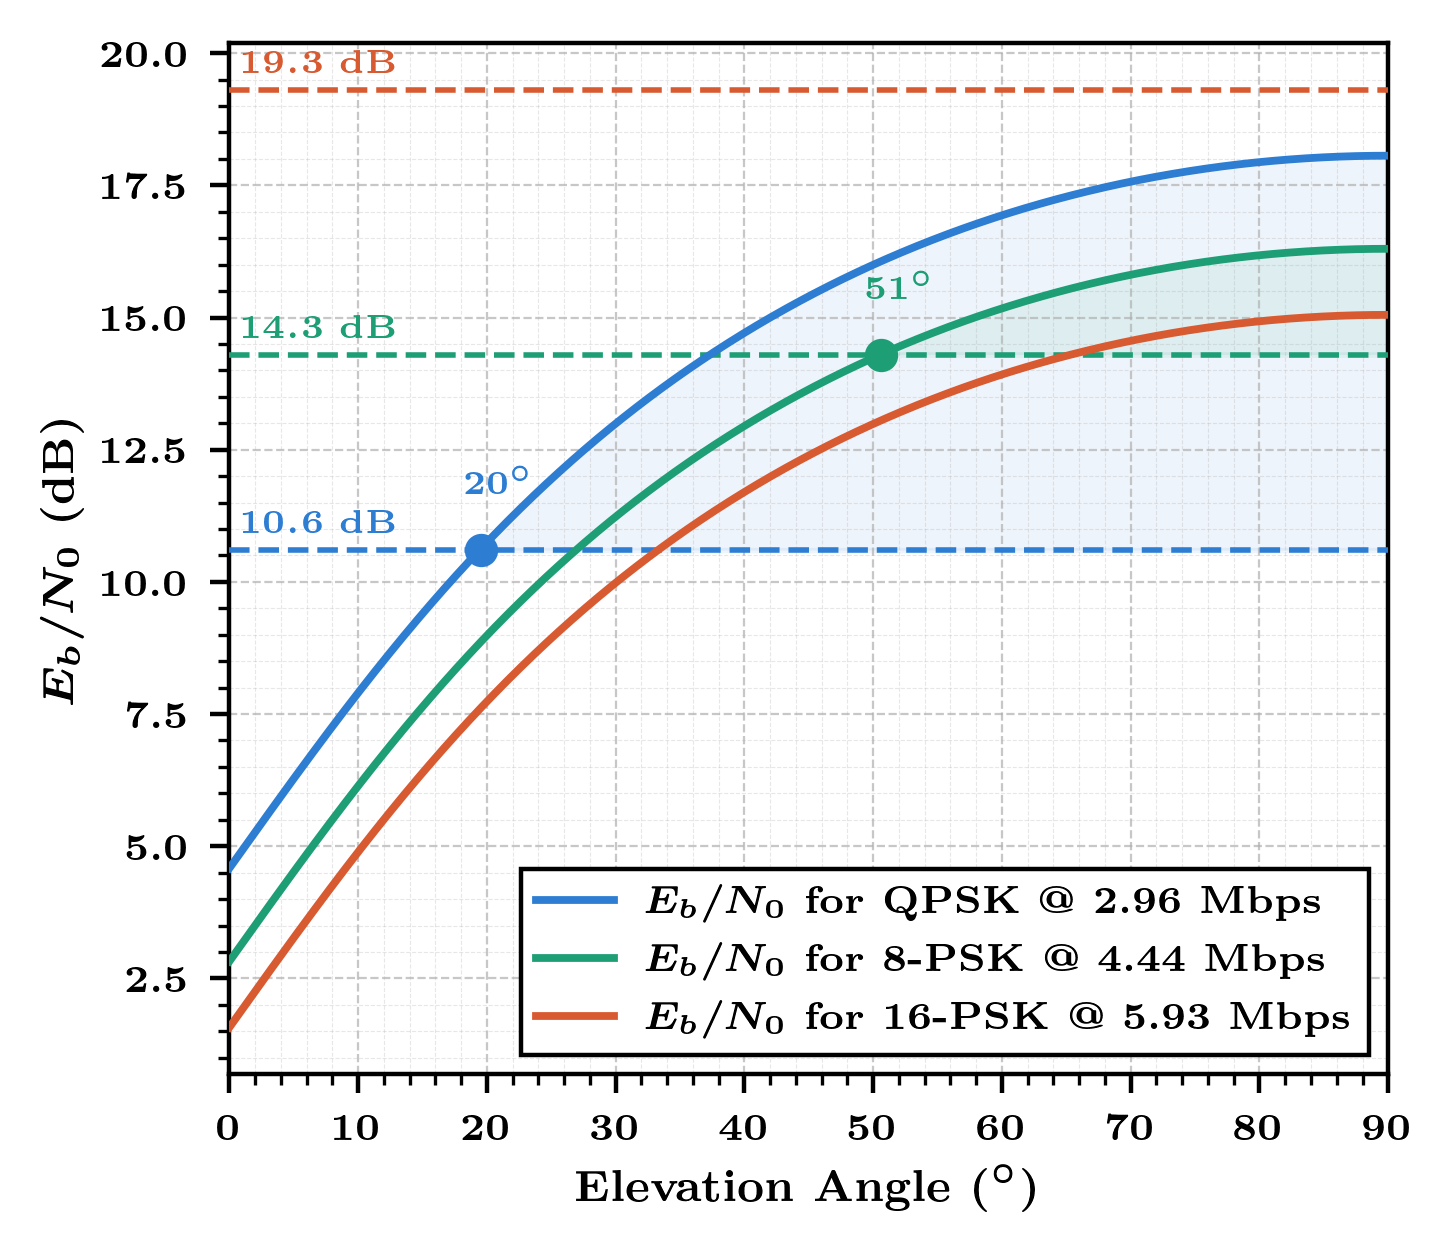
\includegraphics[width=\linewidth]{imgs/link_budget_plot.png}
    \caption{Available $E_b/N_0$ vs. elev. angle for QPSK, 8PSK, and 16PSK over a 2\,MHz BW at 2.2\,GHz. Dashed lines indicate the minimum $E_b/N_0$ required. Filled markers denote the minimum feasible elevation angle for each scheme.}
    \label{fig:link_budget}
\end{figure}

% =========================================================================== %
\subsection{GaN Technology for RF Power Amplifiers}
The demanding requirements of CubeSat RF subsystems, high output power, efficiency, and reliability within tight mass and volume constraints, call for a transistor technology capable of delivering high power density while withstanding the thermal and electrical stresses of space operation. GaN HEMTs have emerged as a strong candidate for this role, and are examined in this section.

GaN is a wide-bandgap semiconductor with a bandgap energy of approximately 3.4\,eV, significantly higher than silicon's 1.12\,eV. This translates into higher breakdown voltages and higher operating temperatures. The higher critical electric field also results in greater electron saturation velocity, which supports operation at microwave and millimeter-wave frequencies \cite{Taur_Ning_2021}.

These transistors are implemented using an AlGaN/GaN heterostructure typically grown on Si, SiC, or sapphire substrates. The lattice mismatch and spontaneous polarization at the AlGaN/GaN interface induce a two-dimensional electron gas (2DEG) with high carrier density and mobility, without doping in the channel region \cite{Ambacher2000}. Most GaN HEMTs, including the device used in this paper, are depletion-mode transistors, meaning the channel conducts by default and a negative gate voltage is required to turn off the device. This characteristic imposes a specific power-up and power-down sequence, the gate bias must be applied before the drain voltage and removed after it, to avoid driving the device into an uncontrolled high-current state that could permanently damage both the transistor and the surrounding circuit. Furthermore, the high power density achievable in GaN devices, with values on the order of 40\,W/mm having been demonstrated \cite{Wu2006}, enables compact implementations well suited to mass and volume-constrained platforms such as CubeSats. The incorporation of field plates at the gate further extends this capability by redistributing the electric field at the gate edge, suppressing peak values and improving both breakdown voltage and linearity \cite{Chiang2012}.

% =========================================================================== %
\subsection{Class AB Operation}
The transistor technology alone does not determine the amplifier's performance, the choice of operating class defines how the device is biased and driven, directly affecting both efficiency and linearity. Class A amplifiers conduct for the full cycle (360\degree), offering the best linearity but a theoretical maximum drain efficiency of only 25\% for a resistive load, a significant limitation for power-constrained platforms such as CubeSats where every milliwatt of dissipated power carries a thermal and energy budget cost. At the opposite extreme, Class C amplifiers conduct for less than half a cycle (below 180\degree), achieving higher theoretical efficiencies but introducing significant nonlinear distortion, incompatible with the constant-envelope modulation schemes discussed in Section~\ref{sec:link_budget}.

Class AB amplifiers conduct for more than half but less than a full cycle. As the conduction angle approaches 180\degree\ (Class B limit), the theoretical drain efficiency approaches 78.5\%, decreasing gradually as the bias is increased toward Class A. This intermediate region allows the designer to balance efficiency, linearity, and device stress within a single topology. Moreover, the power density achievable in GaN devices enables a Class AB design to meet the target output power in a single stage, reducing board area and circuit complexity compared to multi-stage approaches. For CubeSat applications, where both the power budget and signal fidelity are constrained, Class AB provides a practical and robust solution. 

%This choice is consistent with literature on S-Band PAs for satellite and space applications, where Class AB operation has been widely adopted \cite{}.